\documentclass[11pt,a4paper]{article}

% ============================================================
% Packages
% ============================================================

\usepackage[margin=1in]{geometry}
\usepackage{amsmath,amssymb,amsfonts}
\usepackage{bm}
\usepackage{booktabs}
\usepackage{graphicx}
\usepackage{float}
\usepackage{caption}
\usepackage{subcaption}
\usepackage{array}
\usepackage{multirow}
\usepackage{url}
\usepackage{hyperref}
\usepackage{xcolor}
\usepackage{microtype}
\usepackage{setspace}

\onehalfspacing

\hypersetup{
    colorlinks=true,
    linkcolor=blue,
    citecolor=blue,
    urlcolor=blue
}

\graphicspath{{figures/}}

% ============================================================
% Mathematical notation
% ============================================================

\newcommand{\CATE}{\operatorname{CATE}}
\newcommand{\ATE}{\operatorname{ATE}}
\newcommand{\Jaccard}{J}
\newcommand{\ind}{\mathbb{I}}

% ============================================================
% Title
% ============================================================

\title{
\textbf{
Stability-Based Early Stopping for Heterogeneous Effects\\
in Sequential A/B Experiments
}
}

\author{
Mayuri Chatterjee
}

\date{}

% ============================================================
% Document
% ============================================================

\begin{document}

\maketitle

% ============================================================
% Abstract
% ============================================================

\begin{abstract}

Sequential A/B experiments are commonly evaluated using aggregate treatment
effects, although treatment effects may vary substantially across the
population. When treatment effects are heterogeneous, an interim estimate of
the conditional average treatment effect (CATE) can identify a subgroup that
appears to experience meaningful harm even when the estimated harmful
population is not yet stable.

This study investigates a stability-based stopping criterion for sequential
A/B experiments with heterogeneous treatment effects. The proposed criterion
requires both a sufficiently large estimated harmful population and
persistence of that population across consecutive interim analyses. Harm is
defined by an estimated CATE threshold, while population stability is
quantified using Jaccard similarity between consecutive estimated harmful
sets.

A simulation study with 500 replicated experiments compares two heterogeneous
effect structures: a threshold-based effect and a smooth logistic effect.
Each experiment contains 4,000 observations with equal randomized treatment
allocation and is evaluated at six interim sample sizes. The simulation
investigates the probability of stopping, agreement with the final decision,
decision reversal, and stopping sample size.

The results show that requiring stability reduces early stopping and decision
reversal in the threshold-based scenario, where the estimated harmful
population is substantially unstable. At an illustrative Jaccard threshold
of 0.75, stable stopping occurs in 31.4\% of threshold-scenario replicates,
compared with 39.2\% under the naive criterion, while reversal decreases from
20.8\% to 13.8\%. In the smooth-effect scenario, stopping remains highly
probable and reversal remains low. Increasing the Jaccard threshold produces
a systematic trade-off between earlier stopping and decision stability.

These results suggest that the stability of the estimated affected population
can provide useful information beyond the magnitude of an interim treatment
effect when sequential decisions concern heterogeneous treatment effects.

\end{abstract}


% ============================================================
% 1. Introduction
% ============================================================

\section{Introduction}

A/B experiments are often analyzed through an overall treatment effect,
summarizing the difference in outcome rates between treatment and control
groups. Such an analysis is appropriate when the treatment effect is
approximately homogeneous. In many applications, however, the effect of an
intervention can vary substantially across individuals or subpopulations.

The potential-outcomes framework represents this heterogeneity through
individual-level treatment effects and their conditional averages
\cite{rubin1974}. Let $A_i\in\{0,1\}$ denote treatment assignment and let
$Y_i(1)$ and $Y_i(0)$ denote the corresponding potential outcomes. The
individual treatment effect is

\begin{equation}
\tau_i = Y_i(1)-Y_i(0),
\end{equation}

while the conditional average treatment effect is

\begin{equation}
\tau(x)
=
\mathbb{E}\left[
Y(1)-Y(0)\mid X=x
\right].
\end{equation}

The CATE is therefore a function of the observed covariates rather than a
single population-level quantity. Estimation of heterogeneous treatment
effects is consequently relevant when decisions depend on identifying
subgroups for which treatment may be beneficial or harmful
\cite{athey2016}.

Sequential experimentation introduces an additional issue. Suppose that an
experiment is evaluated at several interim sample sizes. The estimated CATE
surface may change as new observations arrive. Consequently, the set of
individuals or covariate values classified as experiencing meaningful harm
may also change.

An early decision based only on the estimated size of this harmful population
may therefore be sensitive to sampling variability. A harmful subgroup
identified at one interim analysis may subsequently shrink, expand, or change
composition.

This motivates a distinction between two questions:

\begin{enumerate}
    \item Is the estimated harmful population sufficiently large to justify
    a stopping decision?
    \item Is the estimated harmful population sufficiently stable across
    interim analyses that the decision is reproducible?
\end{enumerate}

The present study investigates a simple extension of a CATE-based stopping
criterion that explicitly incorporates the second question.

The central idea is to require persistence of the estimated harmful set across
consecutive interim analyses. The stability of two estimated harmful sets is
quantified using their Jaccard similarity. A stopping decision is permitted
only when both the estimated harmful fraction exceeds a prespecified
threshold and the similarity of consecutive harmful sets exceeds a stability
threshold.

The objective is not to derive an optimal sequential testing boundary.
Instead, the purpose of this simulation study is to investigate whether
population-level stability of estimated heterogeneous effects provides useful
additional information for sequential decision-making.

% ============================================================
% 2. Statistical framework
% ============================================================

\section{Statistical framework}

\subsection{Randomized A/B experiment}

Consider a randomized experiment with observations

\begin{equation}
(X_i,A_i,Y_i),
\qquad i=1,\ldots,N,
\end{equation}

where $X_i$ is a baseline covariate, $A_i$ is randomized treatment assignment,
and $Y_i$ is a binary outcome.

Treatment assignment is generated according to

\begin{equation}
A_i\sim\operatorname{Bernoulli}(0.5).
\end{equation}

The marginal average treatment effect is

\begin{equation}
\ATE
=
\mathbb{E}[Y(1)-Y(0)].
\end{equation}

Although the ATE is useful for describing the average effect, the present
analysis focuses on treatment-effect heterogeneity.

\subsection{CATE estimation}

The conditional treatment effect is estimated from a logistic regression
containing treatment, the baseline covariate, and their interaction:

\begin{equation}
\operatorname{logit}
\left\{
P(Y=1\mid A,X)
\right\}
=
\beta_0
+
\beta_1 A
+
\beta_2 X
+
\beta_3 AX.
\end{equation}

For a given covariate value $x$, the fitted probabilities under treatment and
control are

\begin{align}
\widehat p_1(x)
&=
P_{\widehat{\beta}}(Y=1\mid A=1,X=x),\\
\widehat p_0(x)
&=
P_{\widehat{\beta}}(Y=1\mid A=0,X=x).
\end{align}

The estimated CATE is then defined on the probability scale as

\begin{equation}
\widehat{\tau}(x)
=
\widehat p_1(x)-\widehat p_0(x).
\end{equation}

This counterfactual construction allows the estimated treatment effect to be
evaluated for every observation in the interim analysis.

% ============================================================
% 3. Harm definition
% ============================================================

\section{Definition of meaningful harm}

The simulation defines meaningful harm using the estimated CATE threshold

\begin{equation}
\widehat{\tau}(X_i)\leq -0.02.
\end{equation}

The corresponding estimated harmful set at interim analysis $k$ is

\begin{equation}
\widehat{\mathcal H}_k
=
\left\{
i:
\widehat{\tau}_k(X_i)\leq -0.02
\right\}.
\end{equation}

The estimated harmful fraction is

\begin{equation}
\widehat h_k
=
\frac{
|\widehat{\mathcal H}_k|
}{
n_k
},
\end{equation}

where $n_k$ denotes the sample size available at interim analysis $k$.

The basic CATE stopping criterion is therefore

\begin{equation}
\widehat h_k\geq h_0,
\end{equation}

with

\begin{equation}
h_0=0.50.
\end{equation}

Thus, under the naive rule, an experiment is considered eligible for stopping
when at least 50\% of the observations are classified as experiencing
meaningful harm.

% ============================================================
% 4. Stability criterion
% ============================================================

\section{Stability-based stopping criterion}

\subsection{Jaccard similarity}

To quantify the persistence of the estimated harmful population, consider two
consecutive harmful sets,

\[
\widehat{\mathcal H}_{k-1}
\quad\text{and}\quad
\widehat{\mathcal H}_k.
\]

Their Jaccard similarity is

\begin{equation}
J_k
=
\frac{
|\widehat{\mathcal H}_{k-1}
\cap
\widehat{\mathcal H}_k|
}{
|\widehat{\mathcal H}_{k-1}
\cup
\widehat{\mathcal H}_k|
}.
\end{equation}

The statistic satisfies

\begin{equation}
0\leq J_k\leq1,
\end{equation}

with values closer to one indicating greater overlap between consecutive
estimated harmful populations.

\subsection{Stability-enhanced criterion}

The stability-enhanced stopping rule requires

\begin{equation}
\widehat h_k\geq h_0
\end{equation}

and

\begin{equation}
J_k\geq J_0,
\end{equation}

where $J_0$ is the prespecified Jaccard stability threshold.

The resulting rule can therefore be written as

\begin{equation}
\boxed{
\widehat h_k\geq 0.50
\quad\text{and}\quad
J_k\geq J_0.
}
\end{equation}

The analysis examines

\begin{equation}
J_0
\in
\{
0.50,0.60,0.70,0.75,0.80,0.90
\}.
\end{equation}

The value $J_0=0.75$ is used as an illustrative operating point in the main
results. It is not treated as an empirically optimized threshold.

% ============================================================
% 5. Simulation design
% ============================================================

\section{Simulation design}

\subsection{General design}

The simulation consists of 500 replicated experiments. Each experiment
contains

\begin{equation}
N=4000
\end{equation}

observations.

Treatment is assigned independently with probability 0.5. Six interim
analyses are considered:

\begin{equation}
n_k
\in
\{
1000,
1600,
2200,
2800,
3400,
4000
\}.
\end{equation}

The corresponding information fractions are

\begin{equation}
0.25,\;0.40,\;0.55,\;0.70,\;0.85,\;1.00.
\end{equation}

The baseline covariate is generated from a standard normal distribution,

\begin{equation}
X\sim N(0,1).
\end{equation}

Two heterogeneous treatment-effect scenarios are considered.

% ------------------------------------------------------------
% Scenario A
% ------------------------------------------------------------

\subsection{Scenario A: threshold heterogeneity}

The first scenario contains a sharply defined subgroup for which treatment is
harmful.

A subgroup is defined using the upper quartile of the baseline covariate:

\begin{equation}
\mathcal H
=
\left\{
X>q_{0.75}
\right\}.
\end{equation}

The corresponding subgroup contains approximately 25\% of the population.

Under control, the outcome probability is

\begin{equation}
p_0=0.10.
\end{equation}

For observations outside the harmed subgroup, treatment has no effect,

\begin{equation}
p_1-p_0=0.
\end{equation}

Within the harmed subgroup,

\begin{equation}
p_1-p_0=-0.04.
\end{equation}

Thus, the true individual-level treatment effect is

\begin{equation}
\tau(X)
=
\begin{cases}
0,
&
X\leq q_{0.75},
\\[4pt]
-0.04,
&
X>q_{0.75}.
\end{cases}
\end{equation}

The population-average true treatment effect is therefore approximately

\begin{equation}
\ATE\approx -0.01.
\end{equation}

This scenario represents a heterogeneous effect with a relatively sharp
subgroup boundary.

% ------------------------------------------------------------
% Scenario B
% ------------------------------------------------------------

\subsection{Scenario B: smooth logistic heterogeneity}

The second scenario replaces the sharp subgroup boundary with a smoothly
varying treatment effect generated through a logistic functional form.

The treatment effect changes continuously with the baseline covariate rather
than switching abruptly at a fixed threshold. Across the simulated
population, the true CATE is approximately between $-0.062$ and $-0.014$,
with an average effect of approximately

\begin{equation}
\ATE\approx -0.037.
\end{equation}

Unlike Scenario A, the smooth structure does not contain a sharply separated
zero-effect population and harmed subgroup. Consequently, the estimated
harmful population is expected to be more persistent across interim analyses.

The exact data-generating mechanism for this scenario is implemented in the
accompanying R code.

% ============================================================
% 6. Simulation metrics
% ============================================================

\section{Evaluation criteria}

The simulation evaluates four primary characteristics of the stopping rules.

\subsection{Stopping probability}

For each scenario, the stopping probability is the proportion of replicated
experiments for which a stopping criterion is satisfied at any interim
analysis.

\subsection{Agreement with the final decision}

For each replicate, the final interim analysis at $n=4000$ is treated as the
reference decision. Agreement measures whether the sequential stopping
decision is consistent with that final classification.

This is a simulation diagnostic rather than a claim that the final analysis
constitutes a gold-standard clinical decision.

\subsection{Decision reversal}

A reversal occurs when an experiment stops early because the estimated
harmful fraction satisfies the stopping criterion, but the final interim
analysis no longer supports the corresponding harm classification.

This quantity directly measures the instability of early harm-based stopping.

\subsection{Stopping sample size}

The stopping sample size is the first interim sample size at which the
relevant stopping criterion is satisfied.

The stability-enhanced rule is expected to require more information when the
estimated harmful population is unstable.

% ============================================================
% 7. Results
% ============================================================

\section{Results}

\subsection{Evolution of the estimated harmful population}

Figure~\ref{fig:harm_fraction} shows the mean estimated fraction classified
as experiencing meaningful harm across the six interim analyses.

\begin{figure}[H]
    \centering
    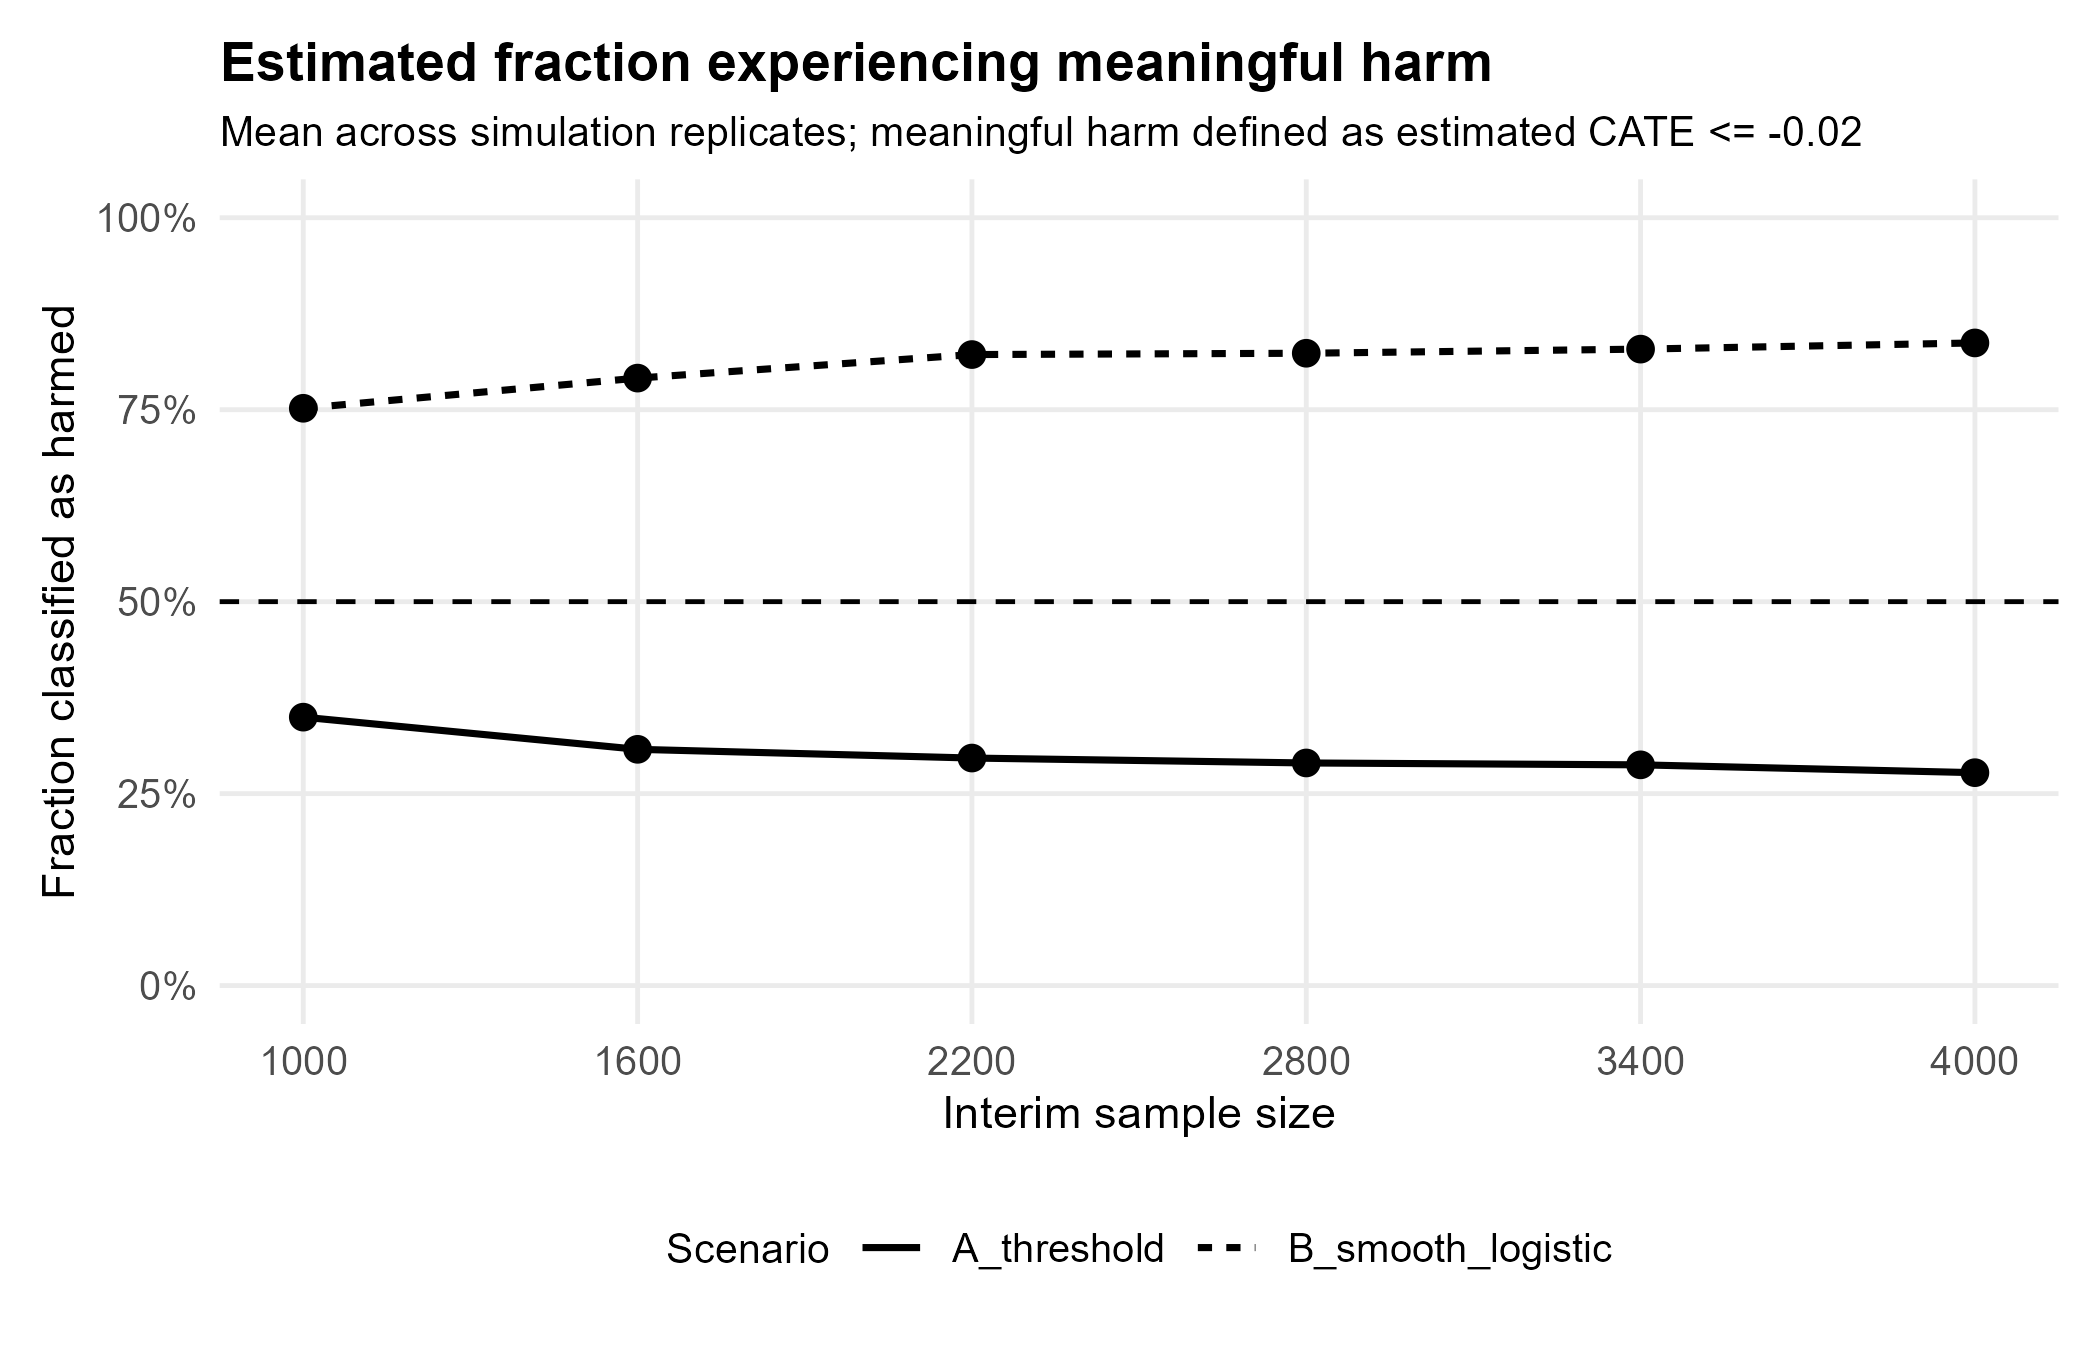
\includegraphics[
        width=0.92\textwidth
    ]{Figure_1_harm_fraction.png}

    \caption{
    Mean estimated fraction of observations classified as experiencing
    meaningful harm across simulation replicates. Meaningful harm is defined
    as an estimated CATE less than or equal to $-0.02$. The horizontal dashed
    line represents the 50\% stopping threshold.
    }
    \label{fig:harm_fraction}
\end{figure}

In Scenario A, the estimated harmful fraction decreases from approximately
35\% at the first interim analysis to approximately 28\% at the final
analysis.

In Scenario B, the estimated harmful fraction remains substantially larger,
increasing from approximately 75\% to approximately 84\%. This difference
between the two scenarios provides a useful contrast between an unstable
threshold-type effect and a smoother heterogeneous effect.

\subsection{Stability of the estimated harmful population}

Figure~\ref{fig:jaccard} shows the Jaccard similarity between consecutive
estimated harmful populations.

\begin{figure}[H]
    \centering
    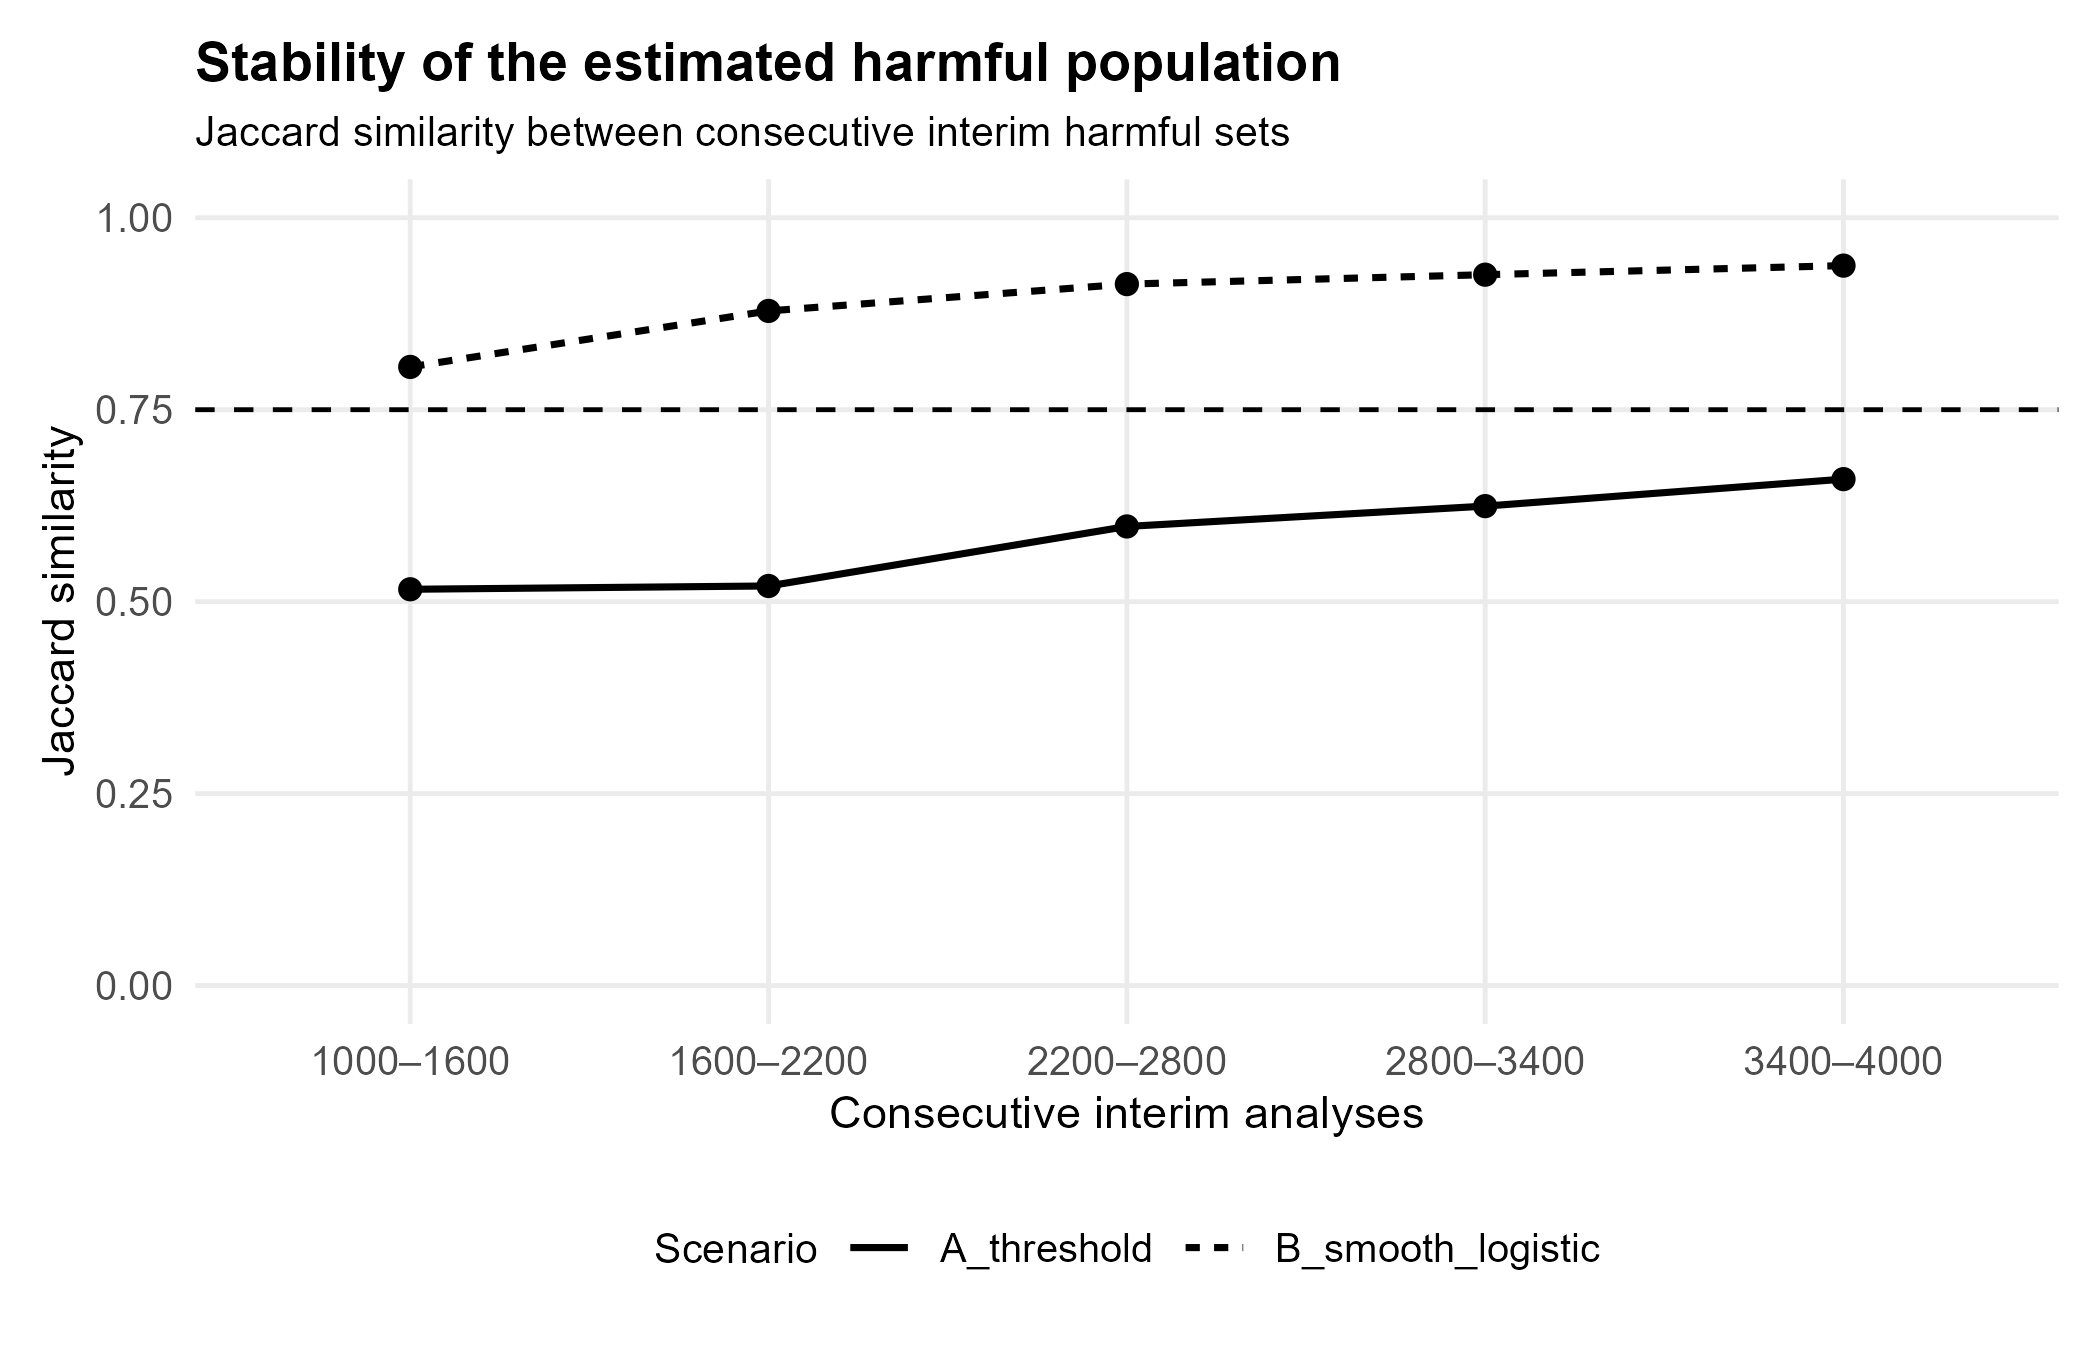
\includegraphics[
        width=0.92\textwidth
    ]{Figure_2_jaccard_stability.png}

    \caption{
    Jaccard similarity between consecutive estimated harmful populations.
    The dashed horizontal line indicates the illustrative stability threshold
    $J_0=0.75$.
    }
    \label{fig:jaccard}
\end{figure}

Scenario A exhibits considerably lower stability. The Jaccard similarity
starts at approximately 0.52 and increases to approximately 0.66 by the final
transition. None of the observed mean similarities reaches the illustrative
threshold of 0.75.

In contrast, Scenario B has substantially higher Jaccard similarity. The
similarity increases from approximately 0.81 at the first transition to
approximately 0.94 at the final transition.

The result indicates that the two scenarios differ not only in the magnitude
of their estimated harmful fractions but also in the persistence of the
estimated harmful population.

\subsection{Sensitivity to the stability threshold}

Figure~\ref{fig:stopping_probability} shows the probability of stopping under
different Jaccard thresholds.

\begin{figure}[H]
    \centering
    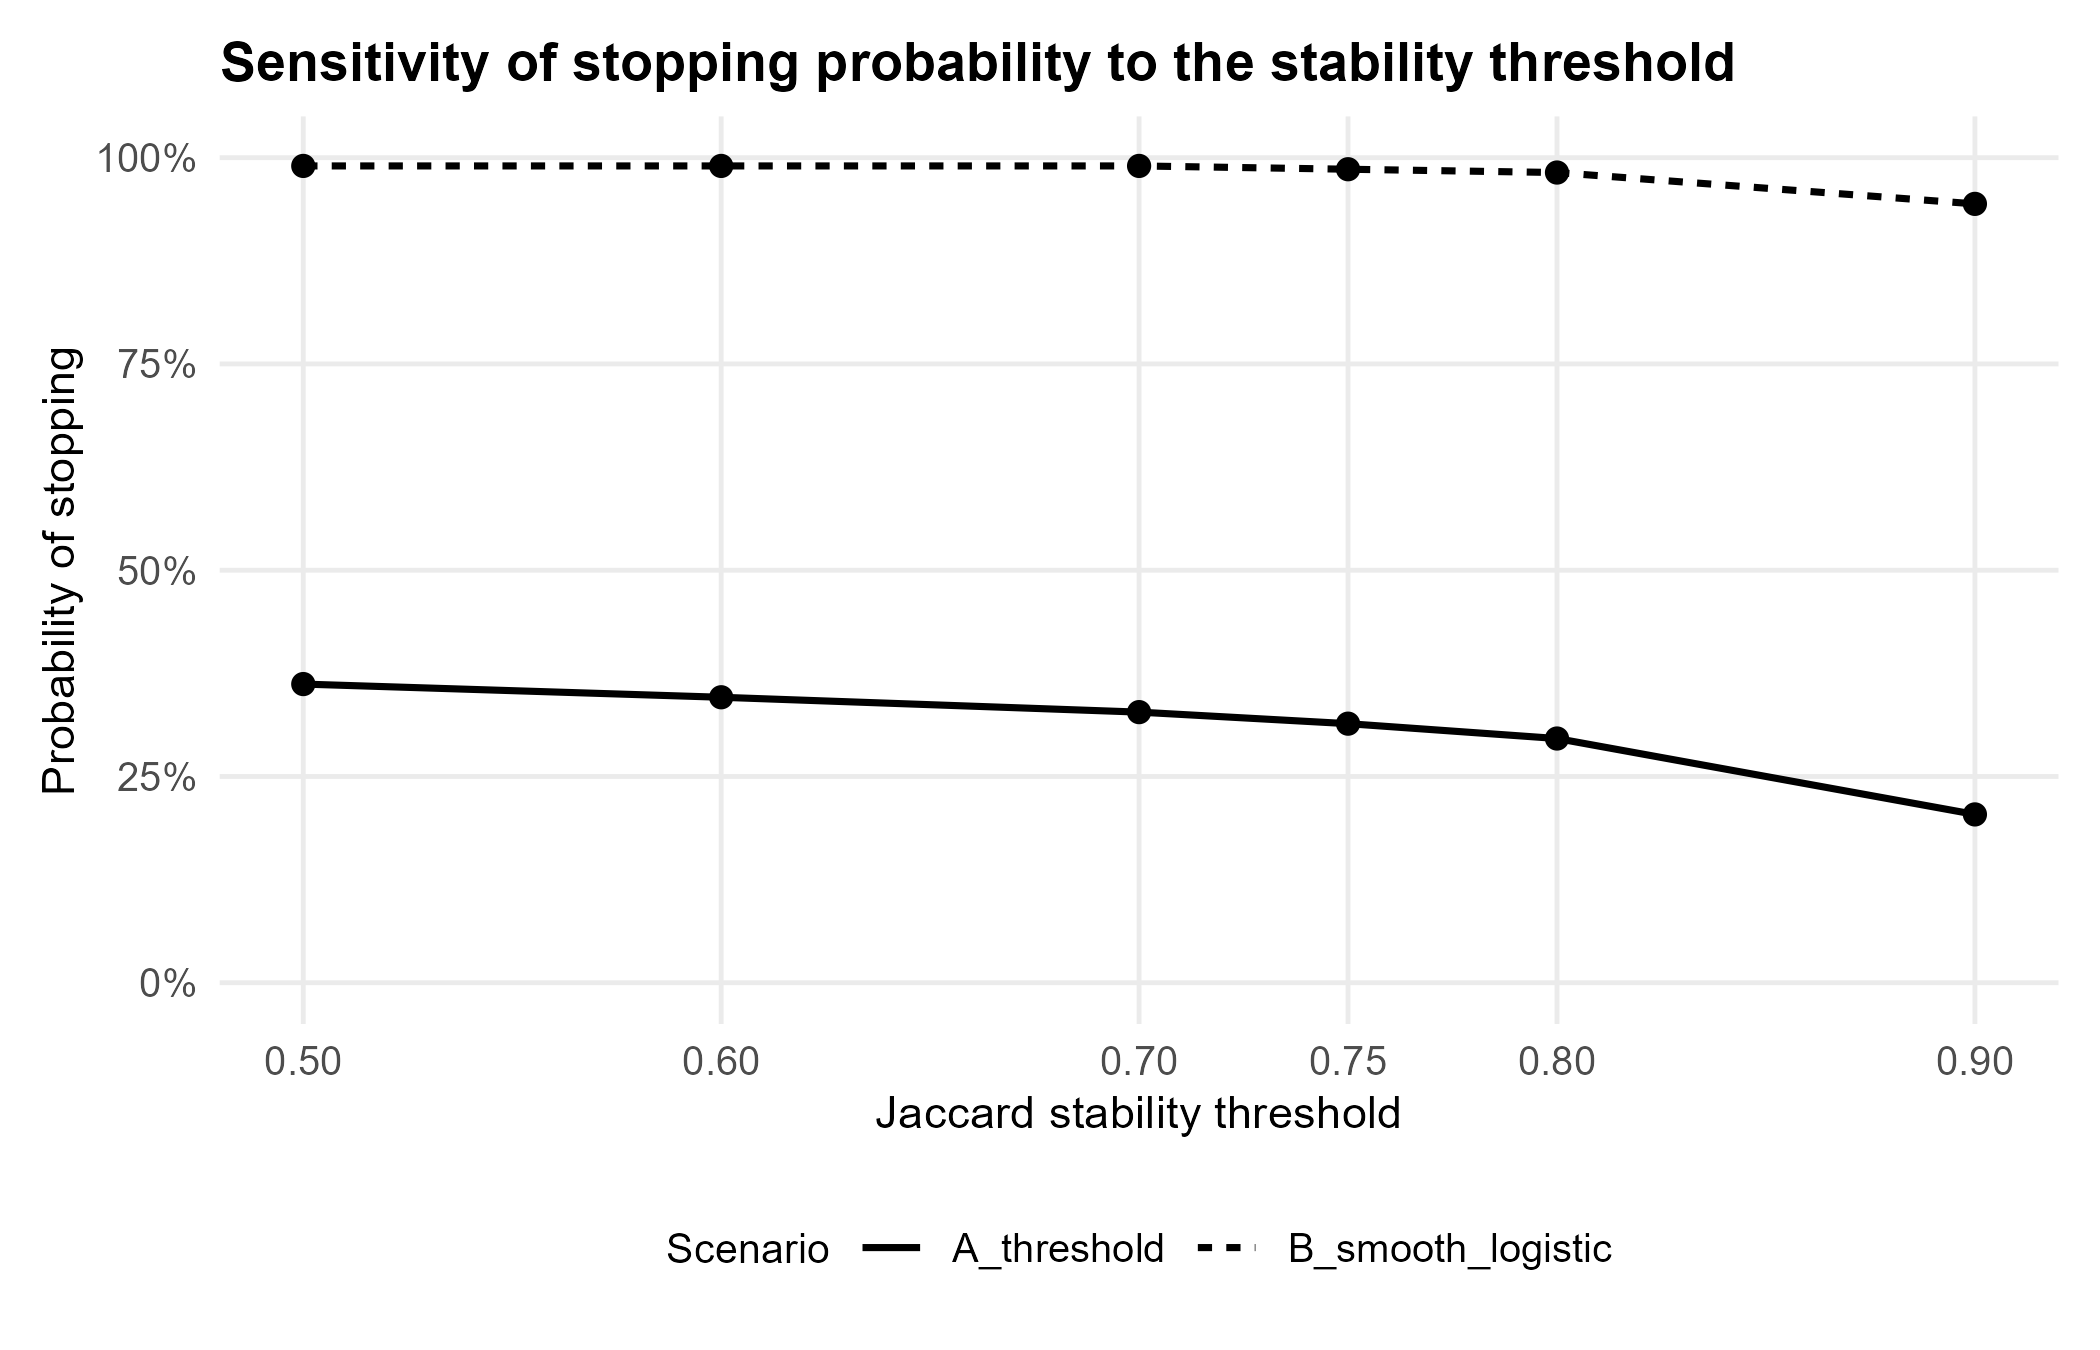
\includegraphics[
        width=0.92\textwidth
    ]{Figure_3_stopping_probability.png}

    \caption{
    Probability of stopping under the stability-enhanced criterion as a
    function of the Jaccard stability threshold.
    }
    \label{fig:stopping_probability}
\end{figure}

For Scenario A, increasing the Jaccard threshold progressively reduces the
probability of stopping. It decreases from 36.2\% at $J_0=0.50$ to 20.4\%
at $J_0=0.90$.

Scenario B is substantially less sensitive. The stopping probability remains
99.0\% at thresholds through 0.70 and decreases to 94.4\% at $J_0=0.90$.

This pattern illustrates the intended role of the stability criterion:
increasing the requirement for persistence primarily suppresses stopping in
the scenario in which the estimated harmful population is unstable.

\subsection{Decision reversal}

Figure~\ref{fig:reversal} presents the probability of decision reversal.

\begin{figure}[H]
    \centering
    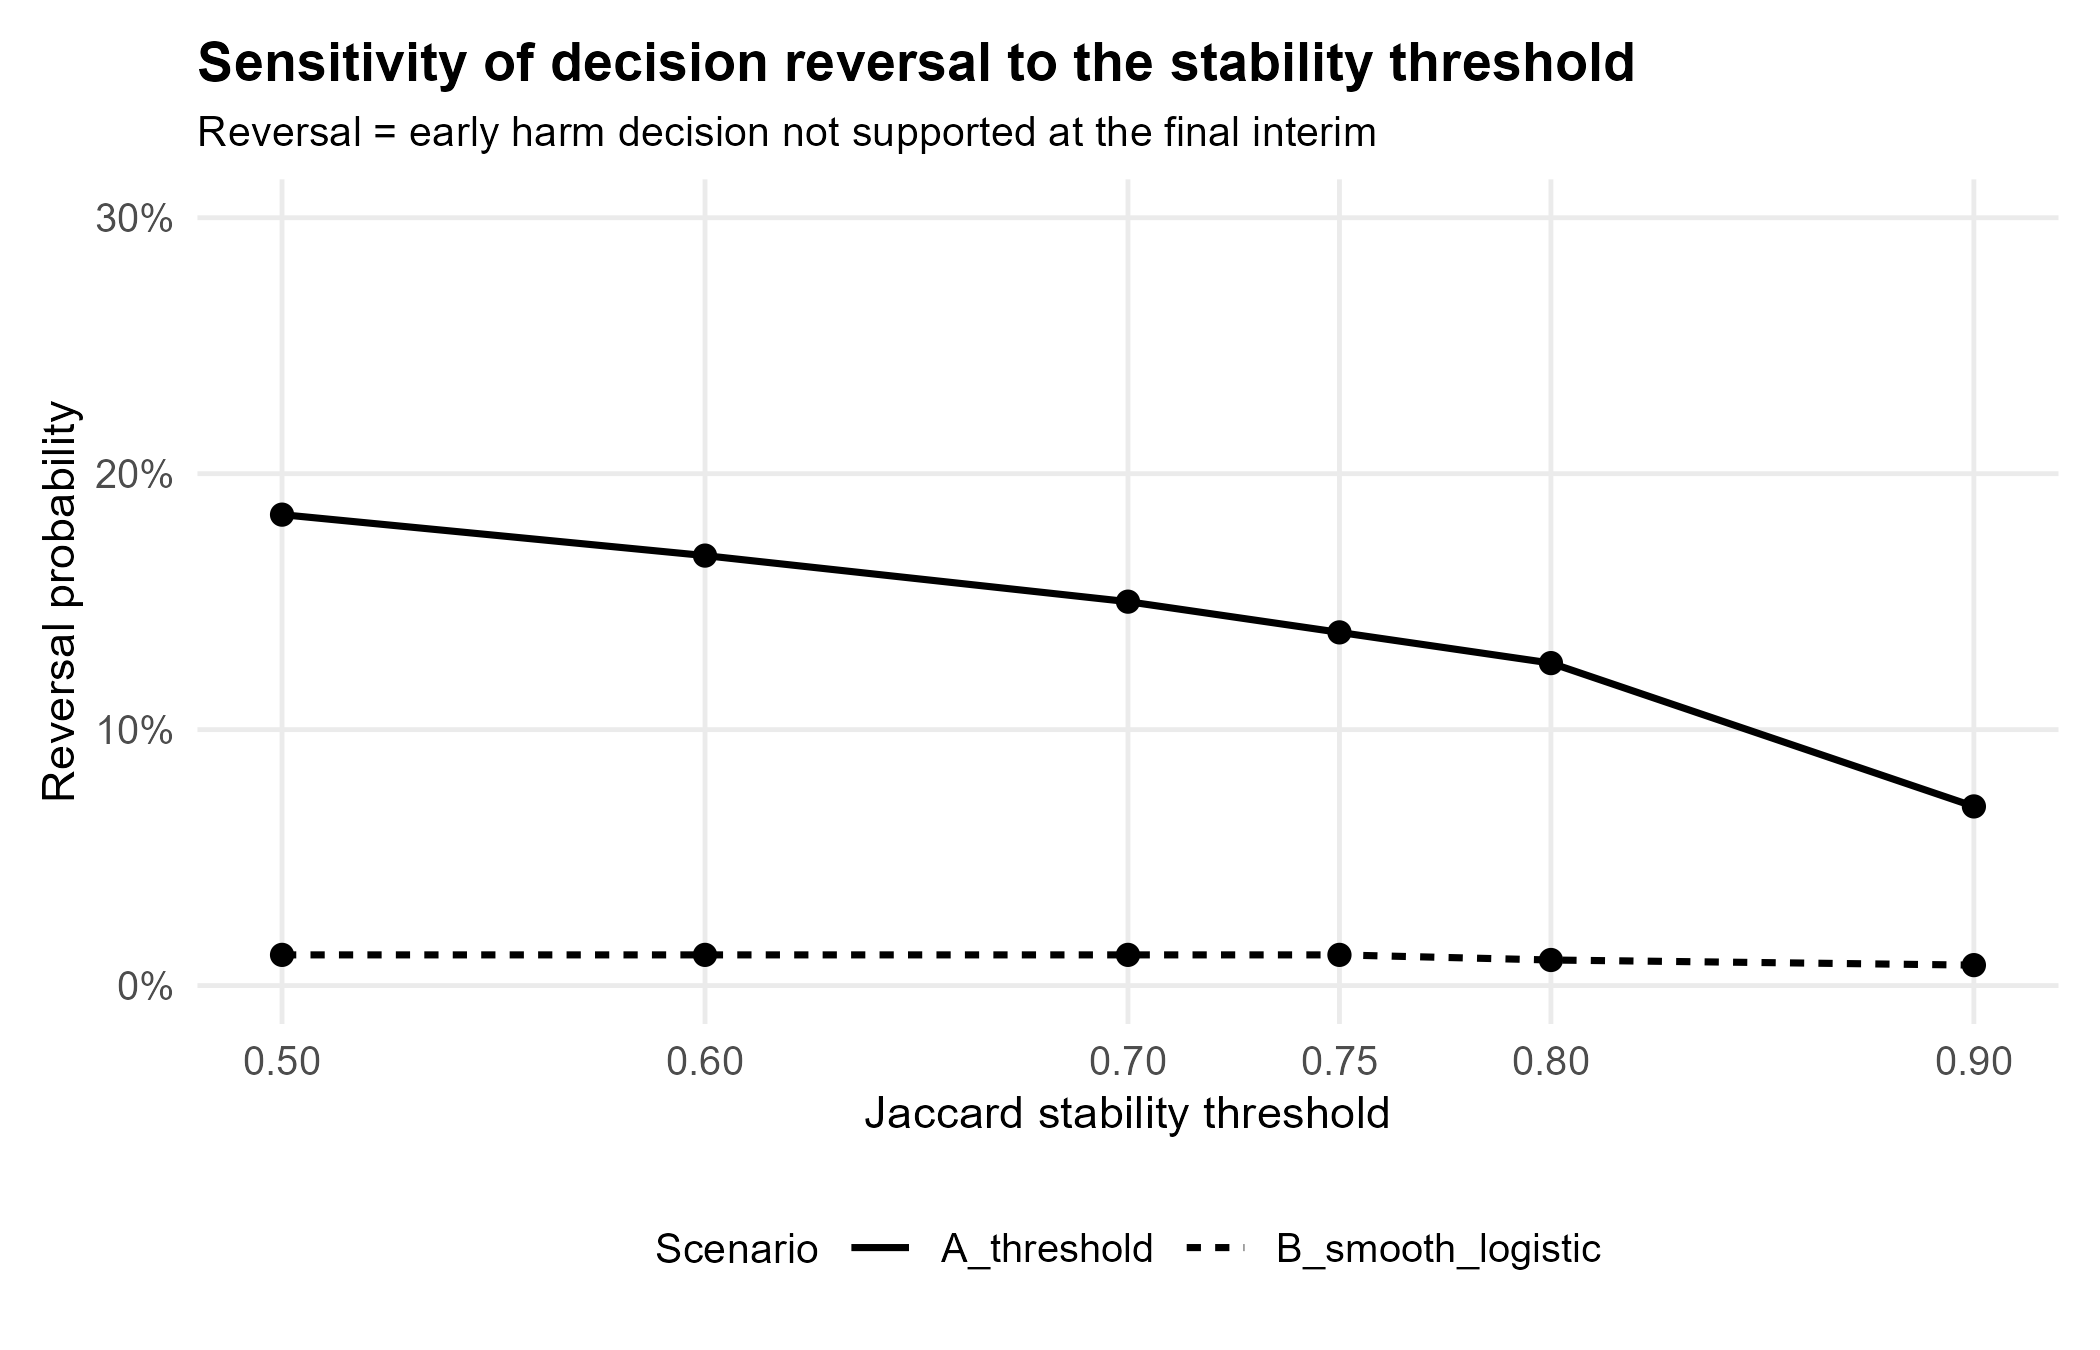
\includegraphics[
        width=0.92\textwidth
    ]{Figure_4_reversal_probability.png}

    \caption{
    Probability of decision reversal as a function of the Jaccard stability
    threshold. A reversal occurs when an early stopping decision based on
    estimated harm is not supported by the final interim analysis.
    }
    \label{fig:reversal}
\end{figure}

The reversal probability decreases systematically for Scenario A as the
stability threshold increases. It falls from 18.4\% at $J_0=0.50$ to 7.0\%
at $J_0=0.90$.

The corresponding probability remains close to 1\% in Scenario B across the
range of thresholds.

Thus, the principal benefit of increasing the stability requirement in the
threshold scenario is a reduction in early decisions that subsequently fail
to persist.

\subsection{Stopping-time trade-off}

The reduction in early stopping is accompanied by an increase in the amount
of information required before stopping.

\begin{figure}[H]
    \centering
    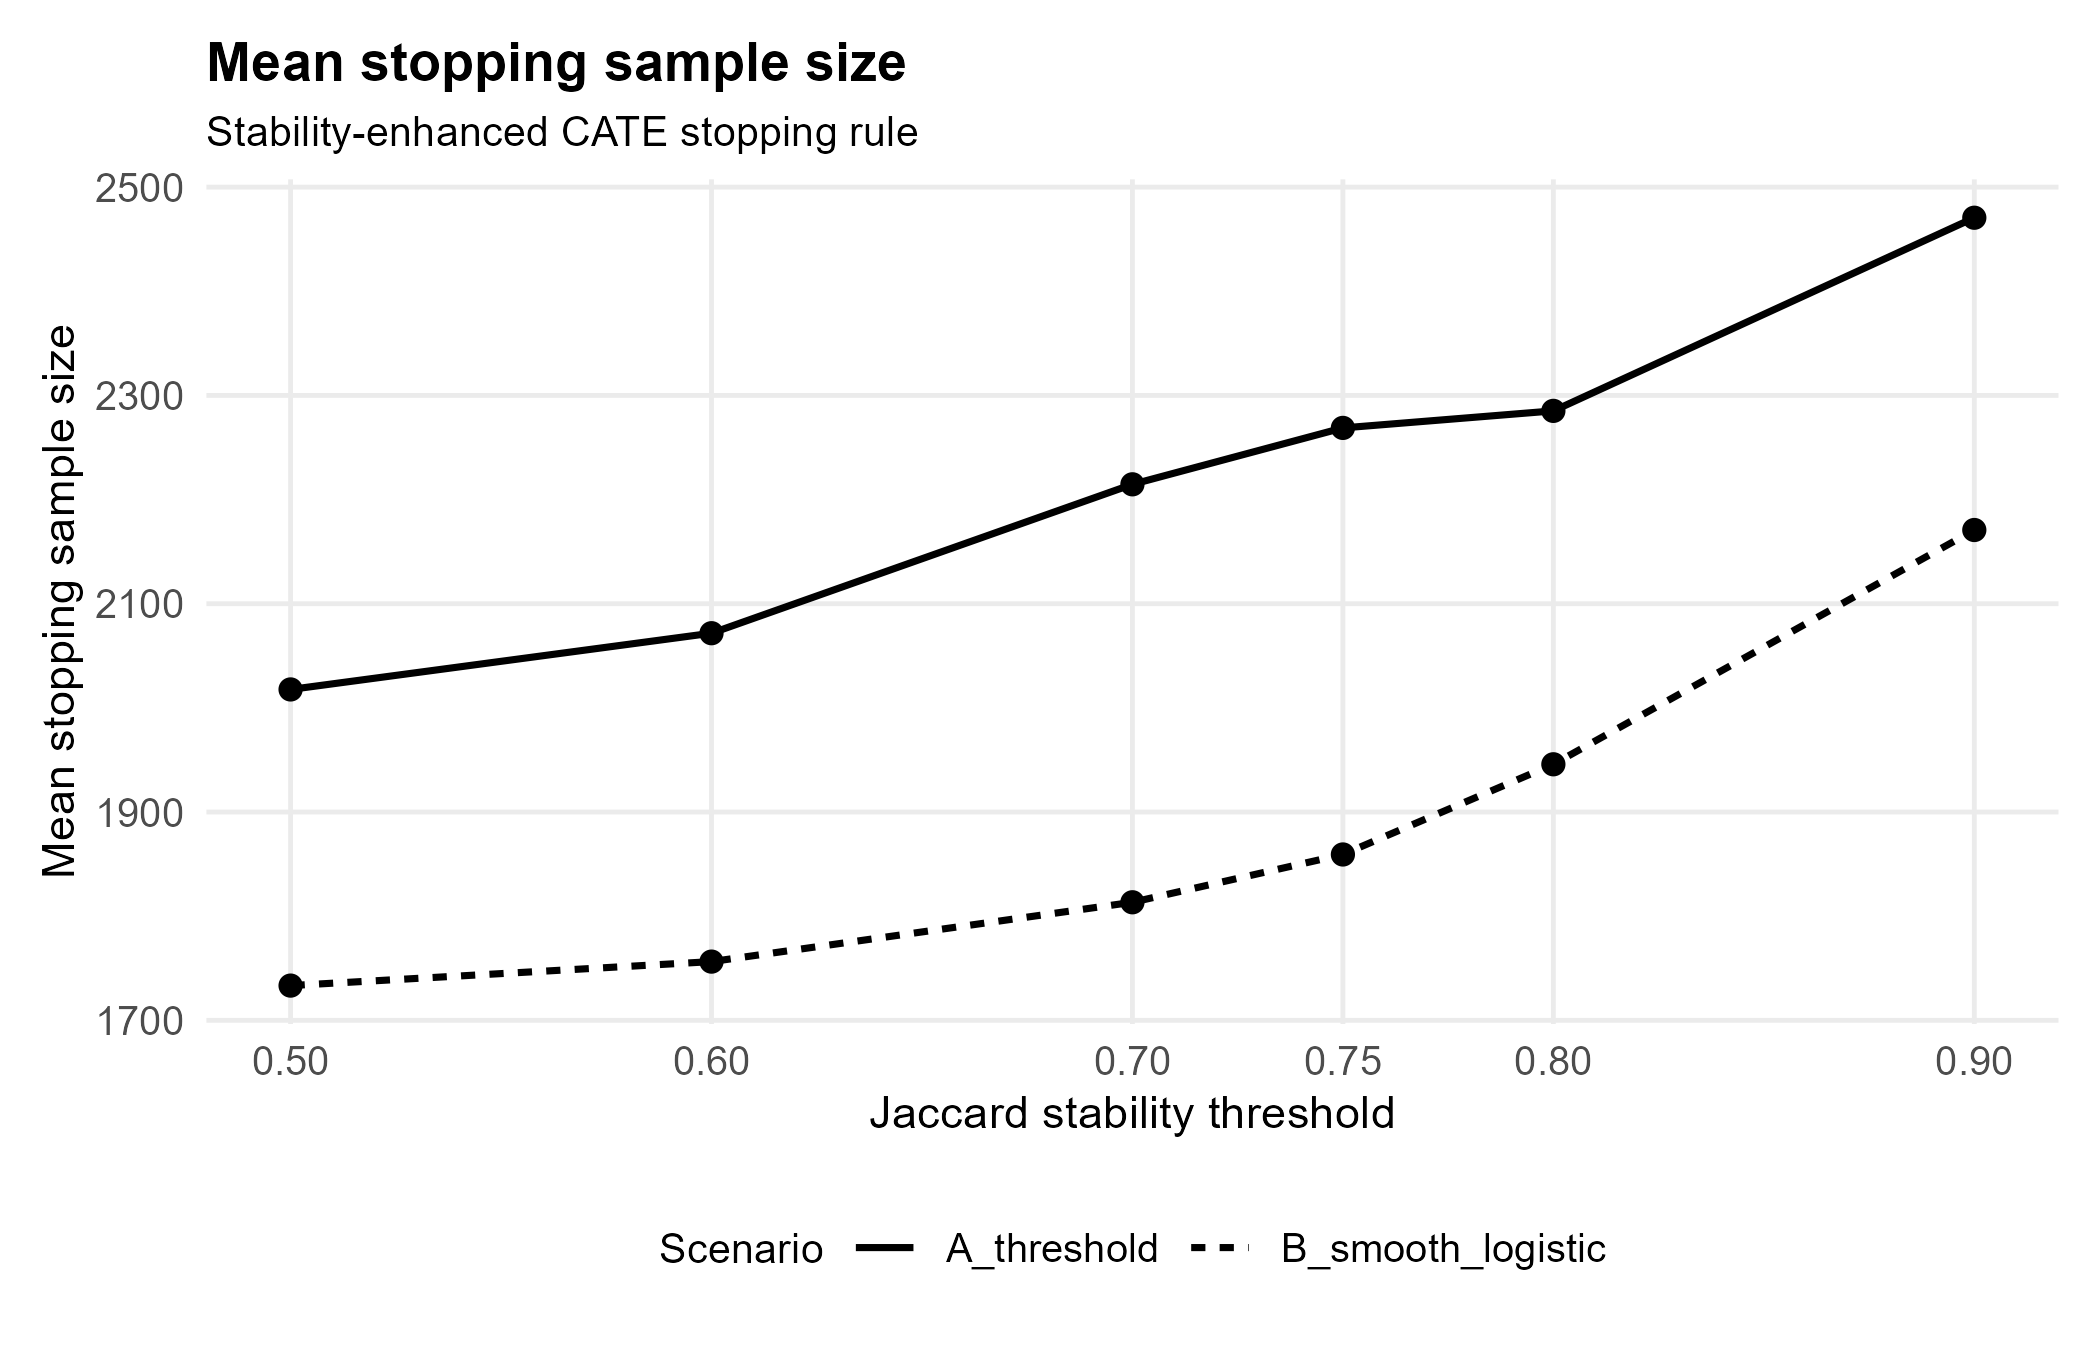
\includegraphics[
        width=0.92\textwidth
    ]{Figure_5_mean_stopping_sample_size.png}

    \caption{
    Mean stopping sample size under the stability-enhanced stopping rule as a
    function of the Jaccard threshold.
    }
    \label{fig:stopping_time}
\end{figure}

For Scenario A, the mean stable stopping sample size increases from
approximately 2,018 at $J_0=0.50$ to approximately 2,471 at $J_0=0.90$.

For Scenario B, the corresponding increase is from approximately 1,733 to
approximately 2,171.

The stability requirement therefore introduces an explicit efficiency versus
stability trade-off: more stringent persistence requirements reduce early
reversal but delay stopping.

% ============================================================
% 8. Main operating point
% ============================================================

\subsection{Illustrative operating point: $J_0=0.75$}

For a more focused comparison, Table~\ref{tab:main_results} summarizes the
results at the illustrative Jaccard threshold

\begin{equation}
J_0=0.75.
\end{equation}

\begin{table}[H]
\centering
\caption{
Stopping performance at the illustrative stability threshold
$J_0=0.75$.
}
\label{tab:main_results}

\begin{tabular}{lcc}
\toprule
& Scenario A & Scenario B \\
\midrule
Naive stopping probability
& 39.2\% & 99.0\% \\

Stable stopping probability
& 31.4\% & 98.6\% \\

Naive agreement with final decision
& 79.2\% & 98.8\% \\

Stable agreement with final decision
& 85.4\% & 98.4\% \\

Naive reversal probability
& 20.8\% & 1.2\% \\

Stable reversal probability
& 13.8\% & 1.2\% \\

Naive mean stopping sample size
& 1,898 & 1,677 \\

Stable mean stopping sample size
& 2,269 & 1,859 \\

\bottomrule
\end{tabular}

\end{table}

For Scenario A, introducing the stability criterion at $J_0=0.75$ reduces
the stopping probability from 39.2\% to 31.4\%. At the same time, agreement
with the final decision increases from 79.2\% to 85.4\%, while reversal
decreases from 20.8\% to 13.8\%.

The corresponding change in Scenario B is considerably smaller. The stopping
probability remains 98.6\%, and the reversal probability remains 1.2\%.

The stable rule therefore changes the sequential behavior most strongly in
the scenario characterized by lower harmful-set stability.

% ============================================================
% 9. Discussion
% ============================================================

\section{Discussion}

The simulation demonstrates a simple but important distinction between
estimating the magnitude of heterogeneous treatment effects and assessing the
stability of the population identified as being affected.

In Scenario A, the estimated harmful population is unstable across interim
analyses. The corresponding Jaccard similarities are substantially below the
illustrative threshold of 0.75. A stopping rule based only on the harmful
fraction can consequently stop at an interim analysis even when the estimated
harmful classification is not persistent.

Requiring a minimum degree of population stability makes the stopping rule
more conservative in this setting. The principal effect is not merely to
reduce the number of stopping decisions. It is to reduce decisions that do
not remain supported at the final interim analysis.

Scenario B provides a contrasting case. The estimated harmful population is
much more stable, with Jaccard similarities consistently above approximately
0.80. Consequently, the stability requirement has relatively little effect
on the stopping probability.

This behavior is desirable for the proposed criterion. If the estimated
affected population is already persistent, requiring stability should not
substantially obstruct stopping. Conversely, when the population is unstable,
the additional criterion should delay or prevent early decisions.

The sensitivity analysis also demonstrates that the stability threshold
controls a meaningful operating characteristic. Higher values of $J_0$
reduce reversal probability but increase the average stopping sample size.
There is therefore no universally optimal threshold based on the present
simulation alone.

The threshold $J_0=0.75$ is consequently used only as an illustrative
operating point. The sensitivity analysis is more important than the
particular choice of 0.75 because it shows the qualitative relationship
between stability requirements, reversal, and information requirements.

% ============================================================
% 10. Limitations
% ============================================================

\section{Limitations}

Several limitations should be emphasized.

First, the simulation uses a single baseline covariate and a relatively
simple logistic CATE estimation model. Real A/B experiments may contain many
covariates, nonlinear interactions, missing data, or model misspecification.

Second, the harmfulness threshold of $-0.02$ and harmful-fraction threshold
of 50\% are simulation parameters rather than universally meaningful
decision boundaries. Their interpretation depends on the application.

Third, the Jaccard threshold is not selected through an optimality criterion.
The values considered in the sensitivity analysis are intended to demonstrate
the operating characteristics of the proposed rule rather than establish a
universally appropriate threshold.

Fourth, the simulation evaluates agreement with the final interim analysis
rather than an independent external truth criterion. The final decision is
therefore a reference point for assessing sequential instability, not a
formal gold standard.

Finally, the CATE estimates are obtained from a parametric logistic model.
The behavior of the proposed stability criterion under more flexible
machine-learning estimators remains an important area for future work.

% ============================================================
% 11. Conclusion
% ============================================================

\section{Conclusion}

This simulation study examined a stability-based extension of CATE-driven
early stopping in sequential A/B experiments.

The proposed rule combines two conditions:

\begin{equation}
\widehat h_k\geq h_0
\end{equation}

and

\begin{equation}
J_k\geq J_0.
\end{equation}

The first condition asks whether a sufficiently large fraction of the
population is estimated to experience meaningful harm. The second asks
whether the estimated harmful population is persistent across consecutive
interim analyses.

The simulations show that these two requirements behave differently under
different forms of treatment-effect heterogeneity. In the threshold scenario,
where the estimated harmful population is substantially less stable, adding
the stability criterion reduces early stopping and decision reversal. In the
smooth logistic scenario, where the estimated harmful population is more
persistent, the additional criterion has a much smaller effect.

At the illustrative threshold $J_0 = 0.75$, the stability-enhanced rule reduces
reversal from 20.8\% to 13.8\% in the threshold scenario, while retaining a high
stopping probability of 98.6\% in the smooth logistic scenario.

The main implication is therefore not that a particular Jaccard threshold is
universally optimal. Rather, the simulation suggests that the stability of
the estimated affected population can be treated as an additional diagnostic
for sequential decisions involving heterogeneous treatment effects.

% ============================================================
% References
% ============================================================

\begin{thebibliography}{9}

\bibitem{rubin1974}
Rubin, D. B. (1974).
Estimating causal effects of treatments in randomized and nonrandomized
studies.
\textit{Journal of Educational Psychology}, 66(5), 688--701.

\bibitem{athey2016}
Athey, S., \& Imbens, G. (2016).
Recursive partitioning for heterogeneous causal effects.
\textit{Proceedings of the National Academy of Sciences},
113(27), 7353--7360.

\bibitem{jennison2000}
Jennison, C., \& Turnbull, B. W. (2000).
\textit{Group Sequential Methods with Applications to Clinical Trials}.
Chapman \& Hall/CRC.

\end{thebibliography}

% ============================================================
% Appendix
% ============================================================

\appendix

\section{Reproducibility}

All simulation experiments and analyses are implemented in R.

The analysis is organized into sequential scripts covering:

\begin{enumerate}
    \item data generation,
    \item CATE estimation,
    \item validation,
    \item repeated sequential simulation,
    \item stopping-rule evaluation,
    \item stability-based stopping,
    \item CATE stability metrics,
    \item stability-threshold sensitivity analysis, and
    \item final figure generation.
\end{enumerate}

The accompanying repository contains the R scripts and generated results
needed to reproduce the figures and numerical summaries presented in this
paper.

The simulation uses a fixed random seed for the initial data-generation
experiment, while the repeated simulation framework controls the generation
of replicated experiments.

\end{document}